\section{WGAN}
For building the \gls{WGAN}, the generator architecture can be the same as the \gls{DCGAN}, the critic can keep the overall structure of the discriminator, but it must have the weight clipping constraints to it's parameters. Besides this, the loss function of both the generator and critic must be replaced by the Wasserstein loss as described in \autoref{sub:wgan}.

As the results will show, this type of \gls{GAN} was the hardest to produce good results, many experiments were made in order to find viable hyperparameters, but it still was unable to produce comparable results to the other techniques. Also, per recommendation of the original authors \cite{wasserstein2017}, the RMSProp optimizer was used in these experiments as the momentum of the Adam optimizer may hurt convergence.

\subsection{MNIST}
Training the \gls{WGAN} on the \gls{MNIST} dataset produced the results seen in \autoref{fig:wgan_mnist_metrics}. These results show a high variability on training with different hyperparameters, and none of them were able to reach similar results with previous techniques.

In order to better see the impact of the hyperparameters chosen it is helpful to make different highlights of these results. \autoref{fig:wgan_mnist_clip} shows how different clipping values influenced the results of the tests.

\begin{figure}[hbt]
    \centering
    \caption{Metrics when training a WGAN on MNIST}
    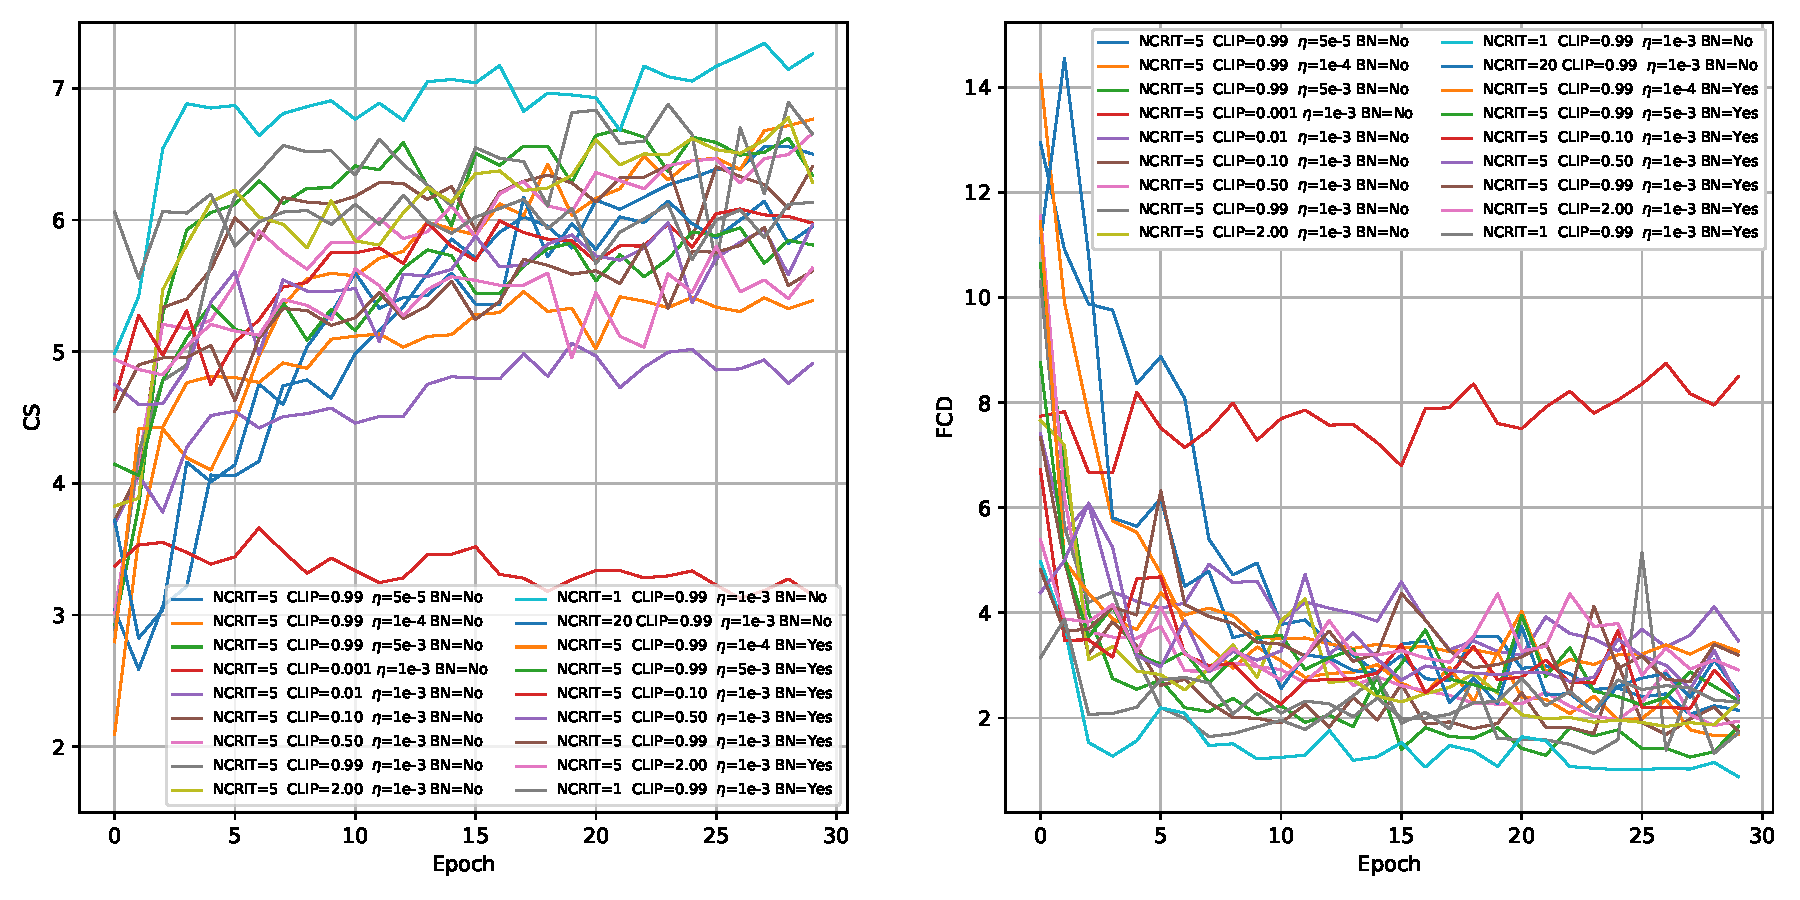
\includegraphics[width=\textwidth]{chapters/Experiments/WGAN/mnist_metrics.pdf}
    \fonte{From the author (2021)}
    \label{fig:wgan_mnist_metrics}
\end{figure}

\begin{figure}[hbt]
    \centering
    \caption{Effects of clipping value when training a WGAN on MNIST}
    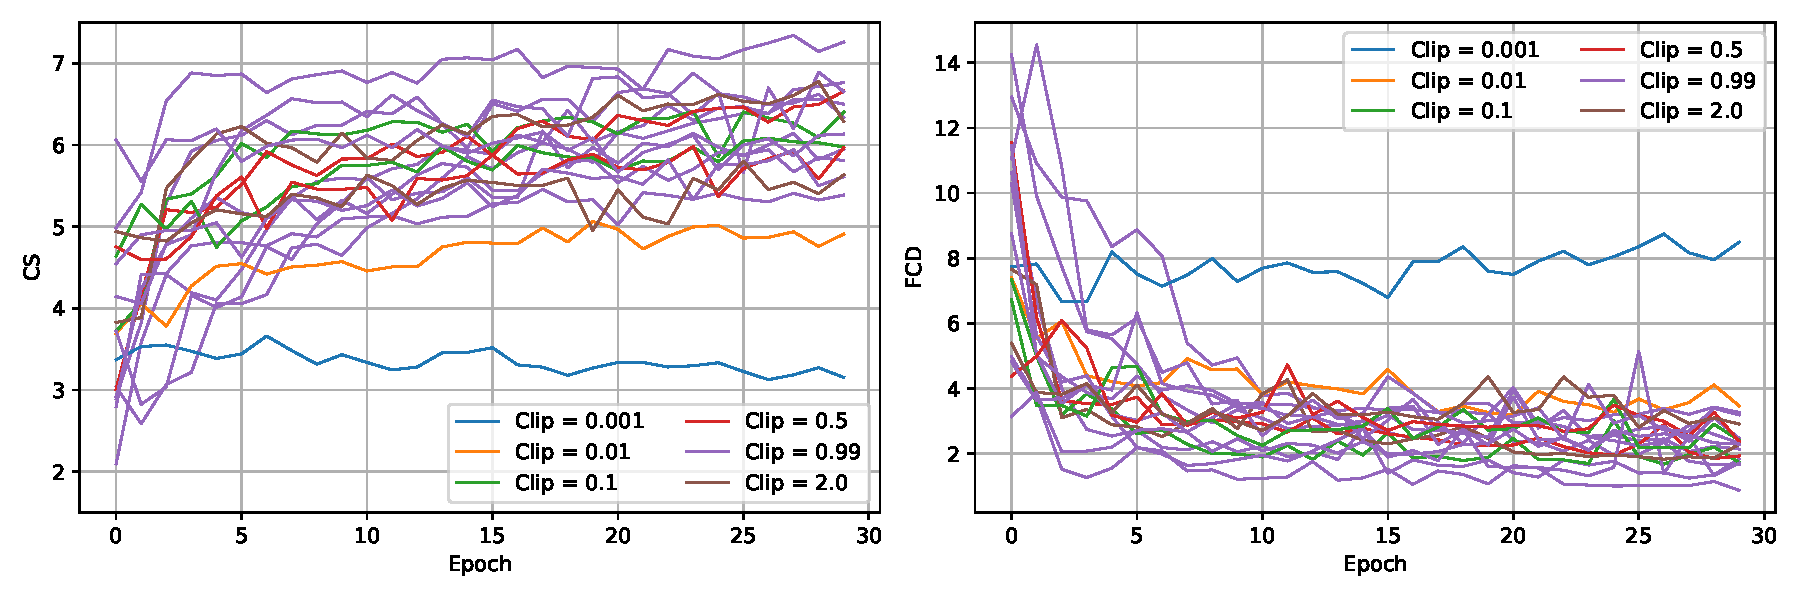
\includegraphics[width=\textwidth]{chapters/Experiments/WGAN/mnist_clipping.pdf}
    \fonte{From the author (2021)}
    \label{fig:wgan_mnist_clip}
\end{figure}

In this case, a clipping value of $0.99$ showed the best results, but even the relatively large range of $0.1$ to $2.0$ still produced similar results overall. The performance only started to decrease for smaller clipping values, this is surprising, since in the original paper proposing \acp{WGAN} it was recommended a value of $0.01$ for clipping \cite{wasserstein2017}. The reason for this may be that the authors trained their models on colored images with higher resolutions and that for these cases, smaller clipping values are beneficial. Whatever the reason, the recommended value produce less favorable results and more experiments would be needed in order to give a more definitive answer.

The use of batch normalization can also be analysed, it's effect can be seen on the highlighted results in \autoref{fig:wgan_mnist_bn_use}. For this case, not using batch normalization has shown better results. 
\begin{figure}[hbt]
    \centering
    \caption{Effects of batch normalization when training a WGAN on MNIST}
    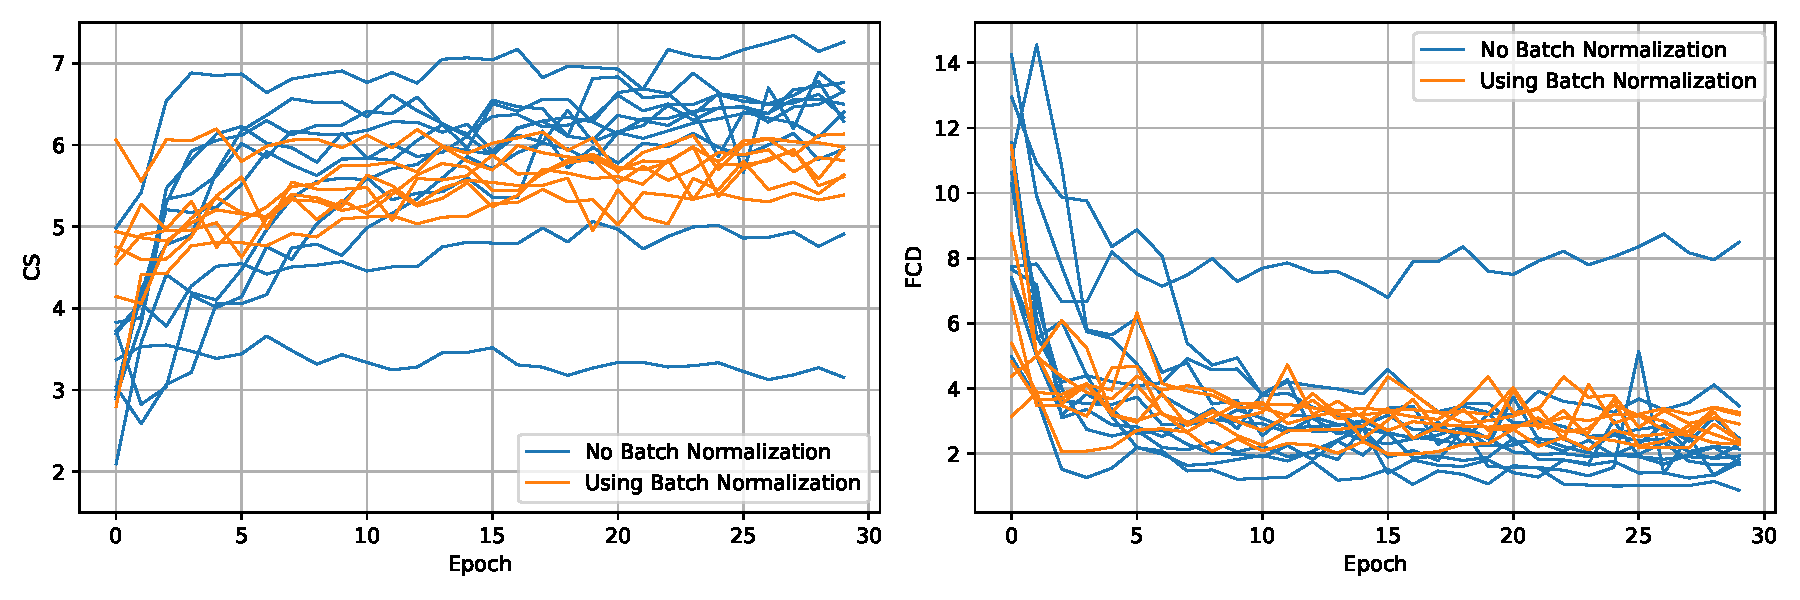
\includegraphics[width=\textwidth]{chapters/Experiments/WGAN/mnist_bn_use.pdf}
    \fonte{From the author (2021)}
    \label{fig:wgan_mnist_bn_use}
\end{figure}

Lastly, the number of critic updates per generator update can be considered. In their original proposal, \textcite{wasserstein2017} argued that training the critic for multiple iterations is something that should be done, since it would only produce more reliable gradients from the critic. However the results shown in \autoref{fig:wgan_mnist_ncrit} question this idea.
\begin{figure}[hbt]
    \centering
    \caption{Effects of number of critic iterations when training a WGAN on MNIST}
    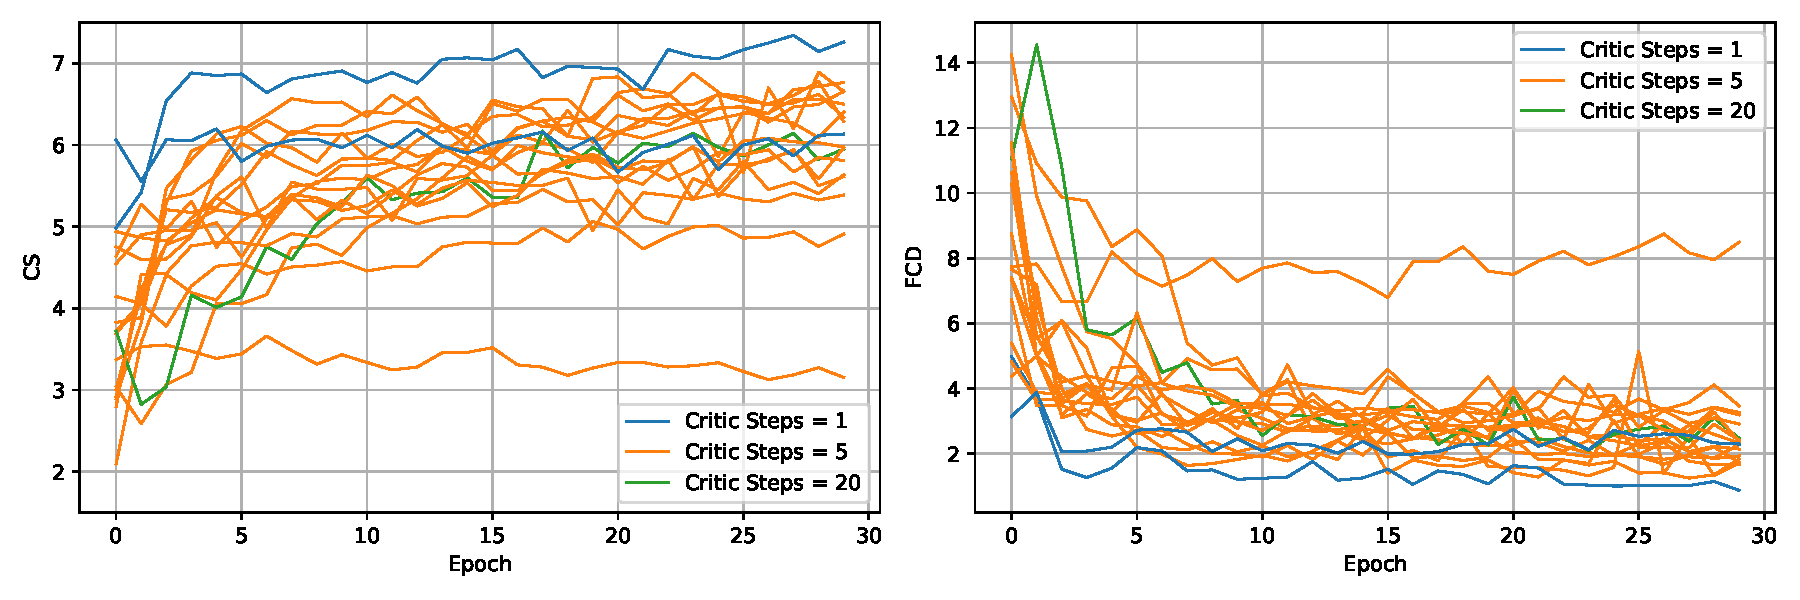
\includegraphics[width=\textwidth]{chapters/Experiments/WGAN/mnist_ncrit.pdf}
    \fonte{From the author (2021)}
    \label{fig:wgan_mnist_ncrit}
\end{figure}

For the experiments made, the actual best policy was to train the critic just as much as the generator. In fact, training for more iterations seemed to reduce the performance, as the test for $20$ critic iterations had one of the lowest performances, beating mainly the methods that were hurt by the use of batch normalization and low clipping values.

One of the reasons for this is similar to the argument made for the batch sizes, just as bigger batches make fewer updates to the networks per epoch, so do larger number of critic iterations. Since the critic must be updated multiple times in order to update the generator once, then more iterations will mean that the generator is updated less. This may give more reliable gradients, but the cost is that the training becomes significantly slower; one alternative could be using fewer iterations when the training starts and the gradients do not need to be very precise, while gradually increasing them as training progresses.

The samples produced for the best model (\texttt{NCRIT=1  CLIP=0.99  $\eta$=1e-3 BN=No}) in the experiments are shown in \autoref{fig:wgan_mnist_samples}.
\begin{figure}[hbt]
    \centering
    \caption{Samples when training a WGAN on MNIST}
    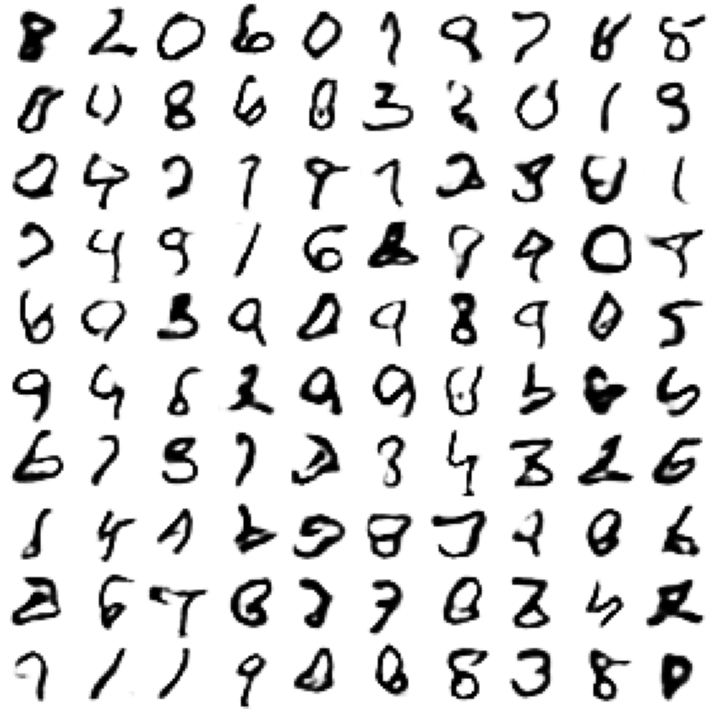
\includegraphics[width=0.5\textwidth]{chapters/Experiments/WGAN/mnist_samples.png}
    \fonte{From the author (2021)}
    \label{fig:wgan_mnist_samples}
\end{figure}


\subsection{Fashion MNIST}
Training the \gls{WGAN} on the Fashion MNIST dataset produced the results seen in \autoref{fig:wgan_fashion_metrics}.
\begin{figure}[hbt]
    \centering
    \caption{Metrics when training a WGAN on Fashion MNIST}
    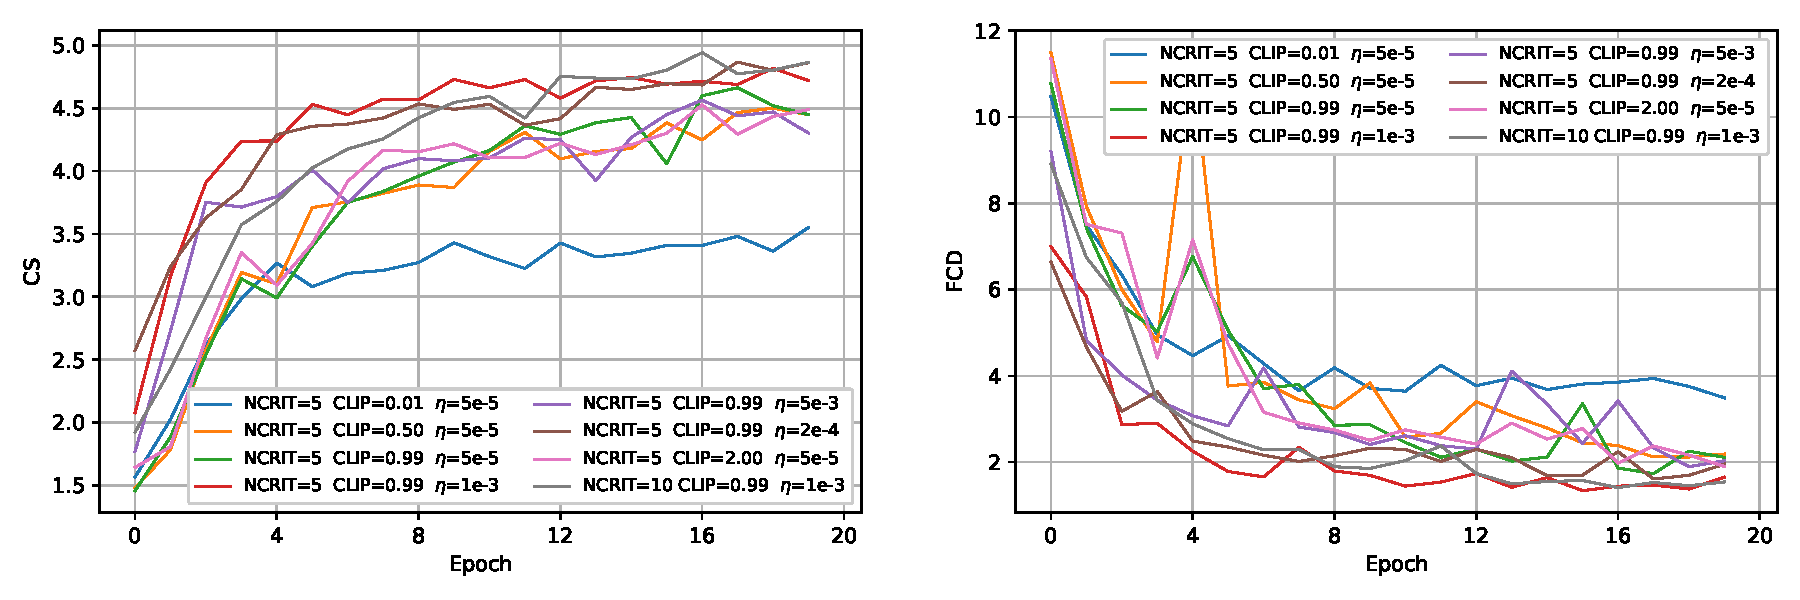
\includegraphics[width=\textwidth]{chapters/Experiments/WGAN/fashion_metrics.pdf}
    \fonte{From the author (2021)}
    \label{fig:wgan_fashion_metrics}
\end{figure}

The clipping values in these results show the same behaviour as seen for the \gls{MNIST} case. However, the effect of the number of iterations for the critic does not seem too strong in this case, it may be because the values tested are relatively closer together, but more tests would be necessary to draw a conclusion.

The learning rate (\gls{learning_rate}) was also experimented on with these and the previous tests with \gls{MNIST}, this hyperparameter is usually something that needs some tuning since it can vary significantly in different types of problems, so it is hard to say anything definitive about it. For the \gls{MNIST} case, highlighting the results by learning rate did not produce very relevant information. For this case, the results may only provide simple insights, but for completion sake they are shown here in \autoref{fig:wgan_fashion_learning_rate}.
\begin{figure}[hbt]
    \centering
    \caption{Effects of learning rate when training a WGAN on Fashion MNIST}
    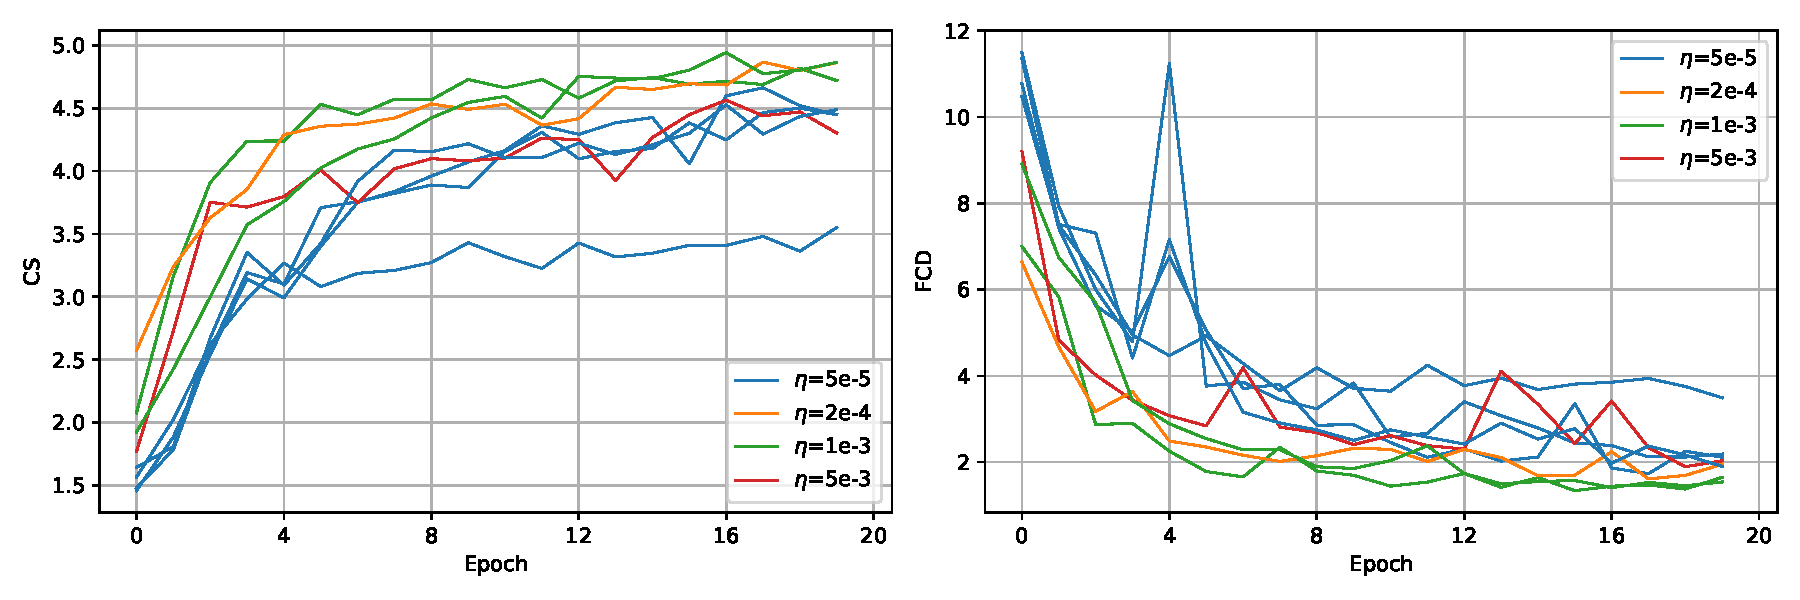
\includegraphics[width=0.9\textwidth]{chapters/Experiments/WGAN/fashion_learning_rate.pdf}
    \fonte{From the author (2021)}
    \label{fig:wgan_fashion_learning_rate}
\end{figure}

The samples generated by the best model for these tests (\texttt{NCRIT=5 CLIP=0.99 $\eta$=1e-3}) are shown in \autoref{fig:wgan_fashion_samples}.
\begin{figure}[hbt]
    \centering
    \caption{Samples when training a WGAN on Fashion MNIST}
    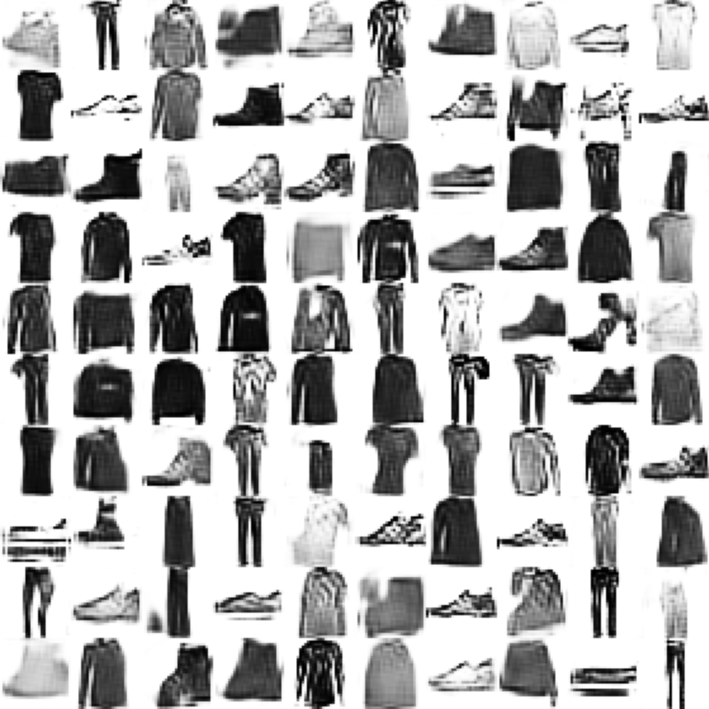
\includegraphics[width=0.5\textwidth]{chapters/Experiments/WGAN/fashion_samples.png}
    \fonte{From the author (2021)}
    \label{fig:wgan_fashion_samples}
\end{figure}
